% Full instructions available at:
% https://github.com/elauksap/focus-beamertheme

\documentclass{beamer}
\usetheme{focus}

\usepackage[utf8]{inputenc}
\usepackage[T1]{fontenc}
\usepackage[french]{babel}

\usepackage{graphics}
\usepackage{graphicx}

\usepackage{pifont}% http://ctan.org/pkg/pifont
\newcommand{\cmark}{\color{example}\ding{51}}%
\newcommand{\xmark}{\color{red}\ding{55}}%
\newcommand{\fmark}{\ding{229}}%
\newcommand{\itemc}{\item[\cmark]}%
\newcommand{\itemx}{\item[\xmark]}%
\newcommand{\itemf}{\item[\fmark]}%

\usepackage{siunitx}

\title{Distribuer l'énergie}
\subtitle{}
\author{ETT - Cours}
\titlegraphic{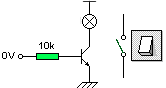
\includegraphics[width=.2\textwidth]{images/transistor_ouvert}}
\institute{IUT de Cachan}
\date{09 novembre 2018}

\begin{document}
    \begin{frame}
        \maketitle
    \end{frame}

    \begin{frame}
        \tableofcontents
    \end{frame}

    \section{Généralités}
    \begin{frame}{La fonction distribuer}
      \centering
      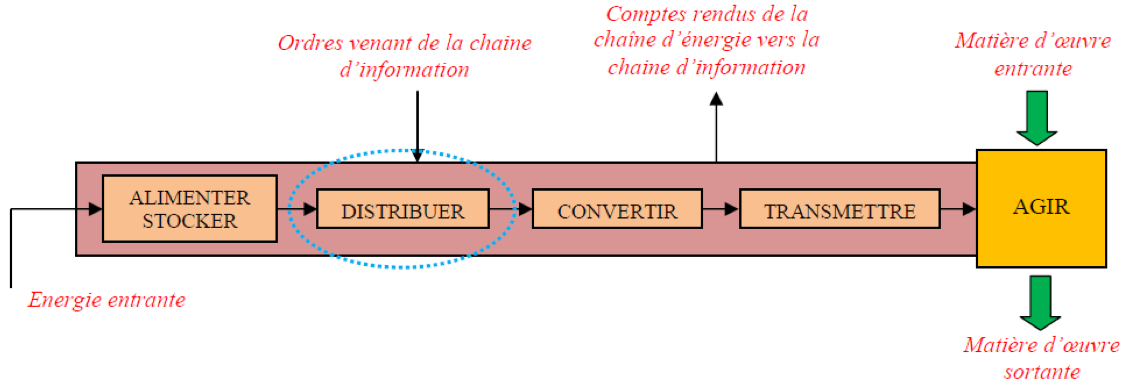
\includegraphics[width=\textwidth]{images/S03_C02}
    \end{frame}

    \begin{frame}{}
      \centering
      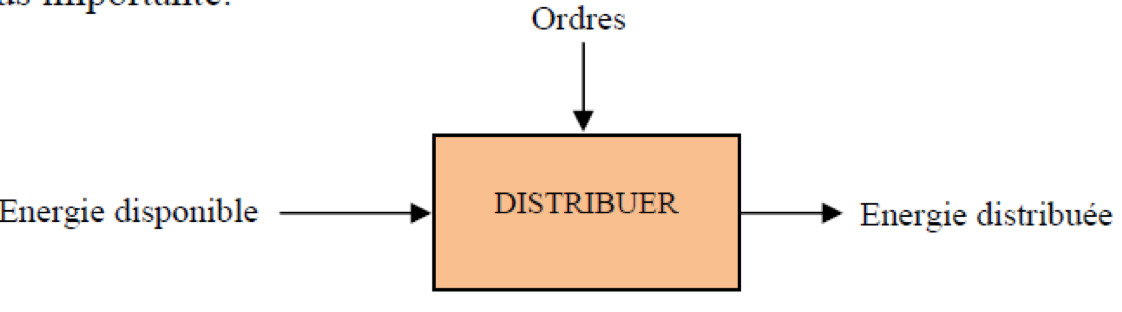
\includegraphics[width=.6\textwidth]{images/distribuer}
    \end{frame}

    \begin{frame}{Définition}
      \begin{alertblock}{Le bloc Distribuer}
        La fonction « Distribuer » de la chaîne d'énergie reçoit des ordre de la part de la chaîne d'information et distribue l'énergie dans le système suivant ces ordres.
      \end{alertblock}

      \visible<2->{\begin{exampleblock}{Propriétés}
        L’énergie est de la même forme en entrée et en sortie. La particularité de cette fonction est qu’une faible énergie de commande venant de la chaîne d’information (ordre) doit entraîner le passage ou non d'une énergie dans la suite de la chaîne d'énergie.
      \end{exampleblock}}
    \end{frame}

    \begin{frame}{Un exemple simple : le robinet}
      \centering
      
\includegraphics[width=.5\textwidth]{images/robinet}
    \end{frame}


\section{Des exemples de solutions technologiques}

\begin{frame}{Le relais électromagnétique}
  \centering
  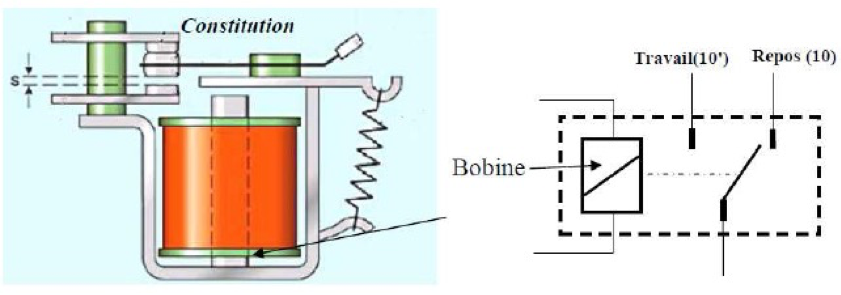
\includegraphics[width=\textwidth]{images/relais_schema}
\end{frame}

\begin{frame}{Relais bistable et monostable}
  \begin{block}{Le relais monostable}
    Un seul état est stable. Lorsque l'on cesse de l'alimenter, le relais retourne spontanément dans cet état.
  \end{block}
  \visible<2->{\begin{block}{Le relais monostable}
    Les deux états sont stables. Il faut apporter de l'énergie au relais pour qu'il change d'état.
\end{block}}
\end{frame}

\begin{frame}{Contacteur}
  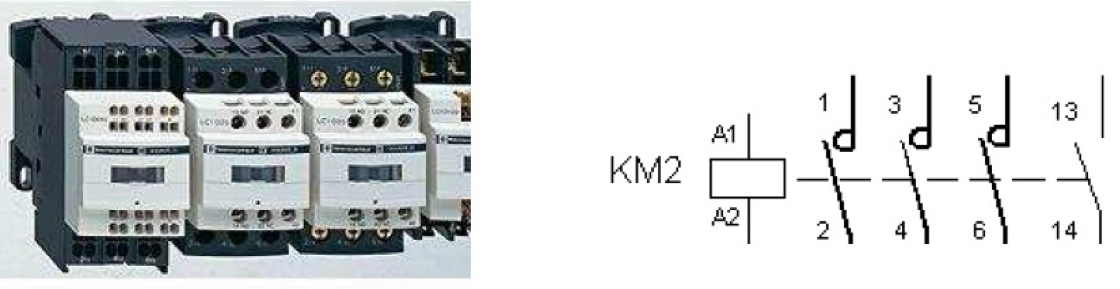
\includegraphics[width=\textwidth]{images/contacteur}
\end{frame}

\section{Les transistors}

\begin{frame}{Les transistors}
  \centering
  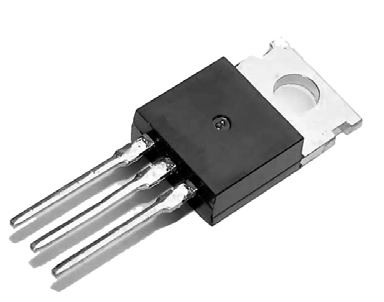
\includegraphics[height=.4\textheight]{images/transistor_img}
  \\
  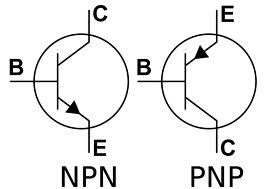
\includegraphics[height=.4\textheight]{images/npn_pnp}
\end{frame}

\begin{frame}{}
  \centering
  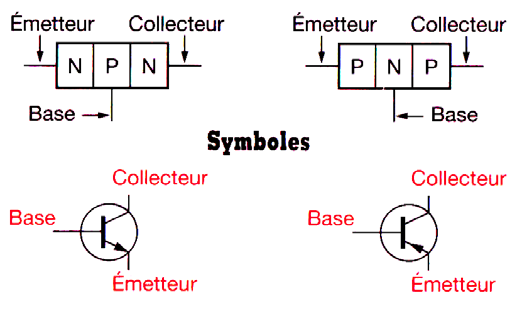
\includegraphics[height=.4\textheight]{images/schema_transistor}
  \visible<2->{\begin{alertblock}{A retenir : }
    Un transistor comporte trois connexions : L’émetteur (E), la base (B) et le collecteur (C).

    L'émetteur est associé à une flèche précisant le sens du courant.

    La base est du côté de la barre.
  \end{alertblock}}
\end{frame}

\begin{frame}{}
  \centering
  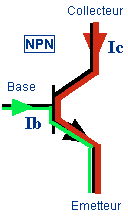
\includegraphics[height=.4\textheight]{images/principe_transistor}
  \begin{alertblock}{Formule d'un transistor}
    $$I_C = \beta I_B$$
  \end{alertblock}
\end{frame}

\begin{frame}{Exemple}
  \centering
  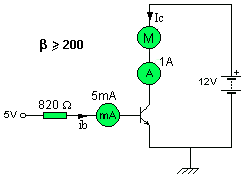
\includegraphics[height=.5\textheight]{images/exemple_moteur}
\end{frame}

\begin{frame}{Fonctionnement en commutation}
  \centering
  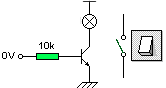
\includegraphics[height=.4\textheight]{images/transistor_ouvert}
\end{frame}

\begin{frame}{Fonctionnement en commutation}
  \centering
  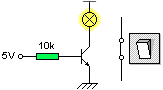
\includegraphics[height=.4\textheight]{images/transistor_ferme}
\end{frame}

\begin{frame}{Transistor MOS}
  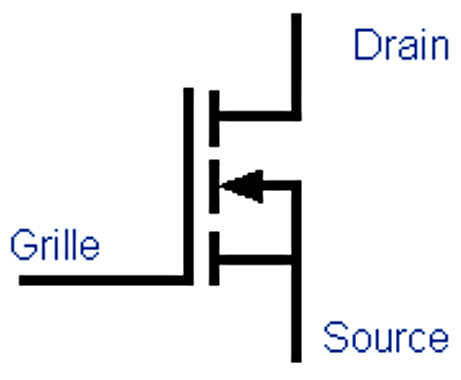
\includegraphics[height=.3\textheight]{images/mos}
  \begin{alertblock}{Principe}
    \textbf{$V_{gs} =0 \Rightarrow$ Transitor bloqué,\hfill $V_{gs} >0 \Rightarrow$ Transitor saturé (passant).}
  \end{alertblock}
\end{frame}

\begin{frame}{Hacheur}
  \centering
  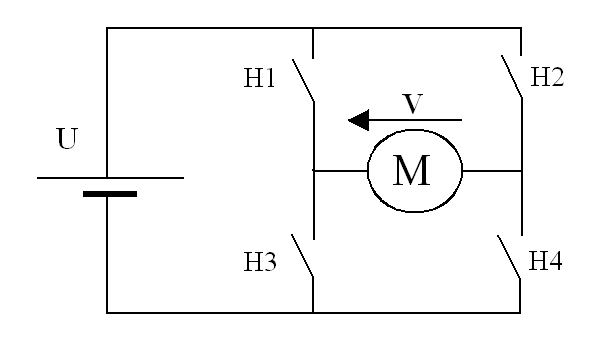
\includegraphics[height=.4\textheight]{images/hacheur}
\end{frame}

\begin{frame}{Onduleur de tension}
  \centering
  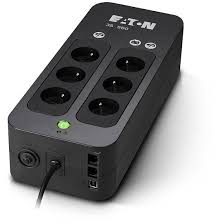
\includegraphics[height=.4\textheight]{images/onduleur}
\end{frame}

\begin{frame}{Redresseur de tension}
  \centering
  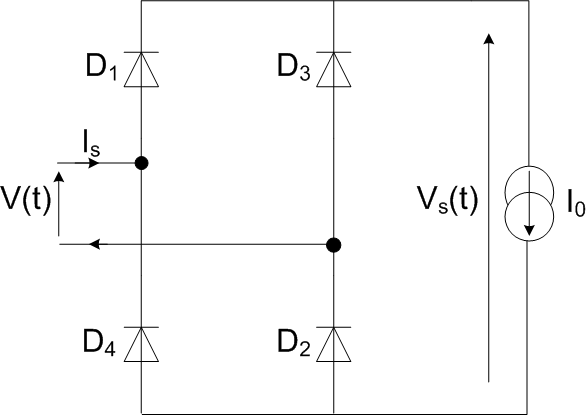
\includegraphics[height=.4\textheight]{images/redresseur}
  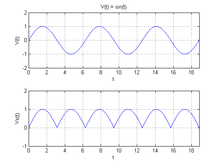
\includegraphics[height=.4\textheight]{images/redresseur_courbes}
\end{frame}
\section{Transformateur électrique parfait}

\begin{frame}{Transformateur électrique}
  \begin{alertblock}{Fonction}
    Un transformateur est un composant permettant d’adapter (augmenter ou abaisser) une tension sinusoïdale. Il est composé de deux bobines de cuivre (inductances) autour d’un circuit magnétique.
  \end{alertblock}
  \centering
  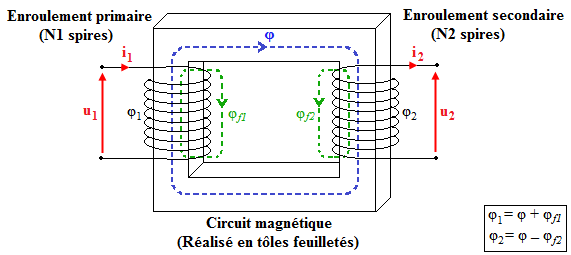
\includegraphics[height=.4\textheight]{images/transfo_principe}
\end{frame}

\begin{frame}{Transformateur électrique}
  \centering
  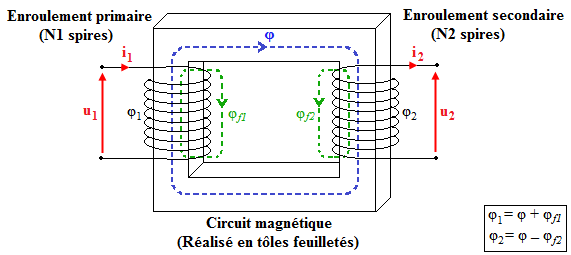
\includegraphics[height=.4\textheight]{images/transfo_principe}
  \begin{alertblock}{Lien tension primaire - Tension secondaire}
    Le courant et la tension dans le circuit secondaire dépendent directement du courant et de la tension dans le circuit primaire. Plus précisément, le \textbf{rapport transformation} $m$ est tel que :
    \begin{center}
        \fbox{$m = \frac{N_2}{N_1} = \frac{U_1}{U_2} = \frac{I_2}{I_1} $}
    \end{center}
  \end{alertblock}
\end{frame}

\begin{frame}{Symbole électrique du transformateur}
  \centering
  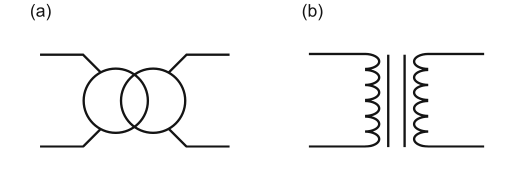
\includegraphics[height=.4\textheight]{images/Symb-transfo}
\end{frame}



    \begin{frame}[focus]
        Applications
    \end{frame}

    \appendix
\end{document}
